% -----------------------------------------------------------------------------
% ########################
% # PREDLOGA ZA POROCILO #
% ########################
%
% @author Iztok Starc
% @date   3. december 2008
%
\documentclass[a4paper,12pt]{report}

% -----------------------------------------------------------------------------
% ####################################################
% # UPORABA PAKETOV - NASTAVITEV JEZIKA in KODIRANJA #
% ####################################################
\usepackage[slovene]{babel}
\usepackage[utf8]{inputenc}
\usepackage{lmodern}
\usepackage[T1]{fontenc}
\usepackage[sc]{mathpazo}
\linespread{1.05}
\usepackage[T1]{fontenc}

% -----------------------------------------------------------------------------
% ######################################
% # VNOS KLJUCNIH PARAMETROV BESEDILA  #
% ######################################

\newcommand{\naslov}     {Implementacija spletne prodajalne in odjemalca za Android}
\newcommand{\prviavtor}  {Primož Hrovat}
\newcommand{\prviindeks} {63150113}
\newcommand{\drugiavtor} {Miha Mazovec}
\newcommand{\drugiindeks}{63150193}
\newcommand{\kraj}       {Ljubljana}

% -----------------------------------------------------------------------------
% ###################
% # UPORABA PAKETOV #
% ###################
\usepackage[a4paper,left=25mm,right=25mm,top=20mm,bottom=30mm,includehead]{geometry}

\usepackage{graphicx, epsfig}

\usepackage{fancyhdr}

\usepackage[
colorlinks=true, linkcolor=blue, citecolor=red,
%
pdftitle={\naslov},
pdfauthor={\prviavtor, \drugiavtor},
pdfsubject={Poročilo seminarske naloge pri predmetu Elektronsko Poslovanje},
pdfkeywords={spletna prodajalna, PHP, SSL, MySQL}, a4paper, pagebackref=true, unicode]{hyperref}

% -----------------------------------------------------------------------------
\begin{document}

% -----------------------------------------------------------------------------
% ##################
% # NASLOVNA STRAN #
% ##################
\begin{titlepage}
	\begin{center}
	{UNIVERZA V LJUBLJANI\\[10pt] 
	FAKULTETA ZA RAČUNALNIŠTVO IN INFORMATIKO}

	\vspace{65mm}

	{\Large\textbf{\naslov}}

	\vspace{10mm}

	{\large Poročilo seminarske naloge pri predmetu\\[10pt] Elektronsko poslovanje}

	\vfill
	\vspace{60mm}

\hspace{20mm}
\begin{minipage}[t]{60mm}
	{\bf Študenti}\\
	{\prviavtor} ({\prviindeks})\\ 
	{\drugiavtor} ({\drugiindeks})\\
\end{minipage}
%\hfill
\begin{minipage}[t]{50mm}
	{\bf Mentor}\\
	David Jelenc
\end{minipage}
%\hspace{20mm}

	\vspace{15mm}

	{	\kraj, \today}
	\end{center}
\end{titlepage}

% -----------------------------------------------------------------------------
% ##################
% # KAZALO VSEBINE #
% ##################

\tableofcontents

% -----------------------------------------------------------------------------
% ############
% # POVZETEK #
% ############
%\begin{abstract}
%\end{abstract}

% -----------------------------------------------------------------------------
% ##################
% # UVOD DOKUMENTA #
% ##################
\chapter{Uvod}

Seminarska naloga je predvidevala izdelavo spletne prodajalne, tako spletne kot mobilne aplikacije za Android. Pri izdelavi sva uporabljala tehnologije PHP, točneje ogrodje Laravel, z namenom spoznavanja tega ogrodja za izdelavo spletnih aplikacij. Mobilni odjemalec temelji na operacijskem sistemu Android, ki je trenutno najbolj razširjen OS na svetu.

% -----------------------------------------------------------------------------
% ###################
% # JEDRO DOKUMENTA #
% ###################

% -----------------------------------------------
\chapter{Navedba realiziranih storitev}
Aplikacija podpira (implementira) naslednje dodatne razširitve:
\begin{enumerate}
    \item Splet:
    \begin{itemize}
        \item Vodenje dnevnika uporabnikov Administrator in Prodajalec.
        \item Registracija strank z uporabo filtriranja CAPTCHA
        \item Registracija strank z uporabo potrditvenega e-maila
        \item Manjše nadgradnje na strani uporabniškega vmesnika (CSS, JS)
        \item Implementacija ocenjevanja artiklov prijavljenega uporabnika ter predstavitev njihove povprečne ocene pri njihovem ogledu.
        \item Implementacija iskanja po artiklih. Iskalnik naj podpira binarno iskanje.
        \item Predstavitev artiklov s slikami. Slike lahko shranite v SUPB ali na datotečni sistem.
    \end{itemize}
    \item Android:
    \begin{itemize}
        \item Osveževanje zaslonov
        \item Prijava in odjava registriranega uporabnika
        \item Pregled artiklov s prijavljenim uporabnikom
        \item Pregled in spreminjanje uporabnikovih podatkov
    \end{itemize}
\end{enumerate}

Delno je implementiran tudi strežniški del za nakupovanje preko vmesnika mobilne aplikacije (košarica, računi...).


% -----------------------------------------------
\chapter{Podatkovni model}

\begin{figure}
    \centering
    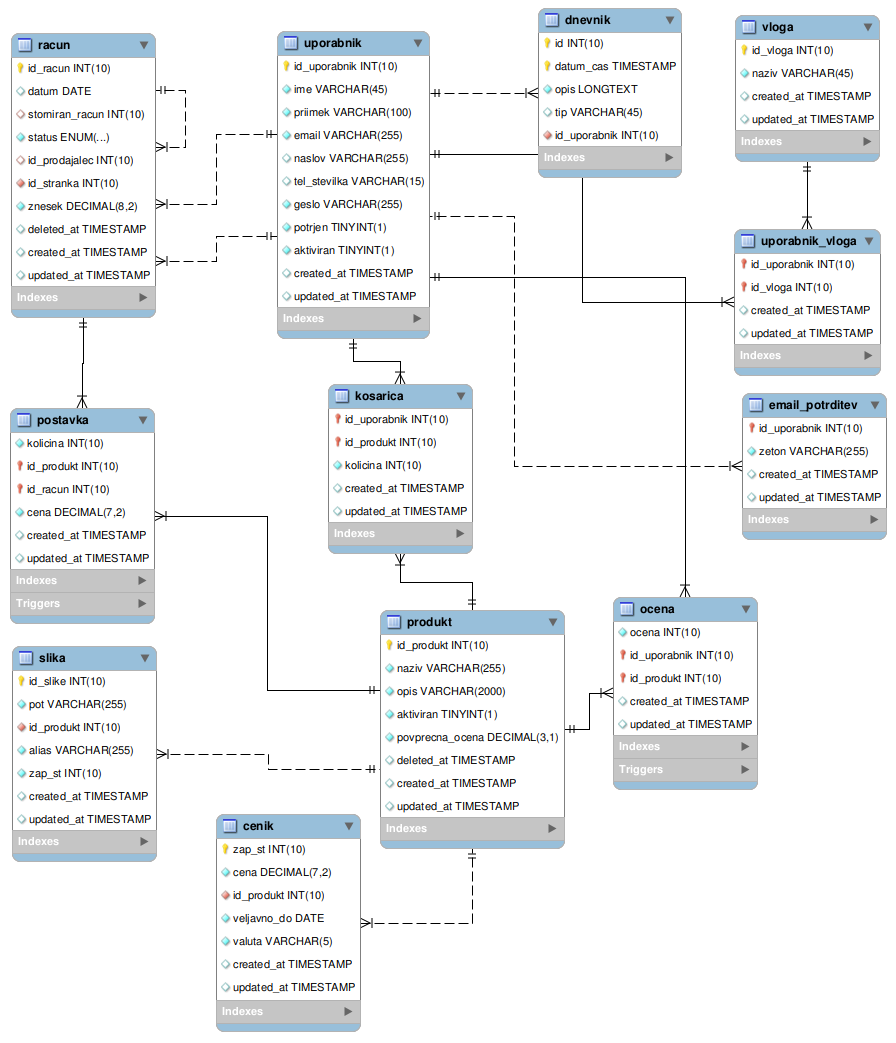
\includegraphics[width=\textwidth]{slike/spletna_trgovina.png}
    \caption{Shema podatkovne baze}
    \label{fig:spletna_trgovina_db}
\end{figure}

Na sliki \ref{fig:spletna_trgovina_db} je prikazana shema uporabljene podatkovne baze. Baza podpira dodeljevanje več vlog uporabnikom, prav tako lahko za posamezen produkt dodamo več cen, upošteva se vedno zadnja veljavna. To lahko koristimo v primeru, da se cena izdelka spremeni, preteklim nakupom pa ne smemo popravljati zneskov, sicer pride do nekonsistence glavne knjige. Baza je načeloma v 3. normalni obliki, z izjemo uporabnikovega atributa naslov, kjer za potrebe naše trgovine ločevanje atributa na nove povezane tabele (naslov, kraj, država) ne predstavlja večjega smisla. Denormalizacija je izvedena tudi na tabeli 'postavka' in 'racun', kjer bazni prožilci sproti popravljajo ceno/znesek, podobno je pri produktu - povprečna ocena se popravlja z baznimi prožilci. 
Relacija 'dnevnik' v atributu 'opis' hrani podatke o zahtevah prodajalcev in administratorja, tip pa predstavlja tip zahtevka HTTP. 'Vloga' služi le kot šifrant za različne tipe vlog: 'administrator', 'prodajalec', 'stranka'.


% -----------------------------------------------
\chapter{Varnost sistema}

Za namene varnosti so strani /admin/* in /prodaja/* dostopne le z uporabo certifikata X.509, potrjenega s strani CA PMCA. PMCA je certifikatna agencija, pripravljena prav za potrebe te spletne aplikacije. Dodatno se pri dostopu /admin in vseh podstrani zahteva uporaba administratorskega certifikata (CN=Administrator). Dodatno se preverjanje uporabnika preverja na strani same aplikacije - poišče se ujemanje elektronskega naslova na podanem certifikatu in tistim, zapisanim v bazi. Od uporabnika se nato zahteva še sam vnos gesla, ki si ga lahko uporabnik po volji spremeni, prav tako je omogočeno urejanje ostalih atributov.

Spletni vmesnik za pregled izdelkov je dostopen preko HTTP in HTTPS protokola, dočim se za prijavo in registracijo izvede preusmerjanje na zavarovan kanal. Vse strani prijavljenega uporabnika so zaščitene s protokolom HTTPS, prav tako vse strani in podstrani /admin in /prodaja.

Vsako preverjanje vnosov s strani uporabnikov je očiščeno html znakov (funkcija htmlspecialchars()), vsi parametri, ki se uporabljajo v poizvedbah SQL se obravnavajo kot parametri in ne kot ukazi (uporaba predpripravljenih poizvedb), kar naj bi preprečevalo vrivanje kode SQL (SQL Injection). S pomočjo ogrodja Laravel se uporablja tudi zaščita pred CRSF napadom.

Vsi dostopi do različnih podstrani, ki zahtevajo prijavo so prav tako ščiteni z uporabo sejnih spremenljivk, ki v primeru nepooblaščenega dostopa izvedejo preusmeritev na stran za prijavo. Pri registraciji uporabnika je zahtevana uspešna rešitev CAPTCHE, katere odziv se preveri na strežniški strani. V kolikor je odziv ustrezen, se uporabnika doda v podatkovno bazo, nadalje pa se mu pošlje potrditveno elektronsko sporočilo z naključno generiranim nizom. S klikom na povezavo se preveri veljavnost niza in v primeru ujemanja uporabniku dovolimo prijavo v trgovino. Pošiljanje elektronskih sporočil je izvedeno preko storitve Mailgun, ki brezplačno omogoča pošiljanje sporočil samo osebam, ki so izrecno dovolile dostavo. Za potrebe demostracije, je v kodi trenutno nastavljen fiksen e-naslov, ki ima dostavo dovoljeno (primoz.hrovat.96@gmail.com). V praksi se ta storitev proti plačilu lahko uporablja nemoteno. Varovanje registracije novih uporabnikov varuje pred zlonamernimi programi - pajki, ki avtomatsko izpolnjujejo nezaščitene spletne obrazce. S CAPTCHO jim delo vsaj otežimo, s potrditvenim sporočilom pa registracijo sicer izvedemo, vendar nepotrjene uporabnike po določenem času pač iz baze izbrišemo.

Za konsistentnost podatkovne baze skrbijo bazni prožilci ter omejitve tujih ključev.

V Android aplikacijo se lahko prijavi le prej registriran uporabnik, ki za prijavo potrebuje e-mail in geslo. V kolikor se skuša prijaviti z napačnim geslom ali napačnim e-mailom ga aplikacija na to opozori, ko pritisne gumb "Prijava". Ko uporabnik vnese veljaven e-mail in geslo, se pošlje zahtevo na strežnik, ki vrne objekt, če je bila prijava uspešna, sicer vrne "null". Vrnjen objekt se shrani v "ApplicationObject", kateri se preverja na vsaki strani aplikacije. V kolikor se uporabnik odjavi iz aplikacije, se njegov objekt nastavi na "null". 

Ob prijavi se uporabniku dodeli seja, ki jo mobilna aplikacija shrani in jo z vsakim naslednjim zahtevkom pošilja strežniku, s čimer se preveri, ali je uporabnik že bil overjen ali ne.

% -----------------------------------------------
\chapter{Izjava o avtorstvu seminarske naloge}

Spodaj podpisani \textit{\prviavtor}, vpisna številka \textit{\prviindeks}, sem (so)avtor seminarske naloge z naslovom \textit{\naslov}. S svojim podpisom zagotavljam, da sem izdelal ali bil soudeležen pri izdelavi naslednjih sklopov seminarske naloge:
\begin{itemize}
    \item načrtovanje in izvedba podatkovne baze
    \item izvedba strežniškega in odjemalskega dela spletne aplikacije za stranko
    \item izvedba strežniškega in odjemalskega dela spletne aplikacije za prodajalca
    \item izvedba strežniškega in odjemalskega dela spletne aplikacije za administratorja
    \item izvedba dodatnih razširitev za spletno aplikacijo (Email, Captcha, dnevnik, CSS, JS, ocenjevanje, iskanje, slike)
\end{itemize}

Podpis: {\prviavtor}, l.r.

\newpage

Spodaj podpisana \textit{\drugiavtor}, vpisna številka \textit{\drugiindeks}, sem (so)avtor seminarske naloge z naslovom \textit{\naslov}. S svojim podpisom zagotavljam, da sem izdelal ali bil soudeležen pri izdelavi naslednjih sklopov seminarske naloge:
\begin{itemize}
    \item načrtovanje podatkovne baze
	 \item izvedba strežniškega in odjemalskega dela spletne aplikacije za stranko
	 \item izvedba odjemalskega dela spletne aplikacije za prodajalca
	 \item izvedba odjemalskega dela spletne aplikacije za administratorja
	 \item izvedba mobilne aplikacije Android
\end{itemize}

Podpis: {\drugiavtor}, l.r.

\newpage

% -----------------------------------------------
\chapter{Zaslonske slike - spletna aplikacija}

\begin{figure}[h]
    \centering
    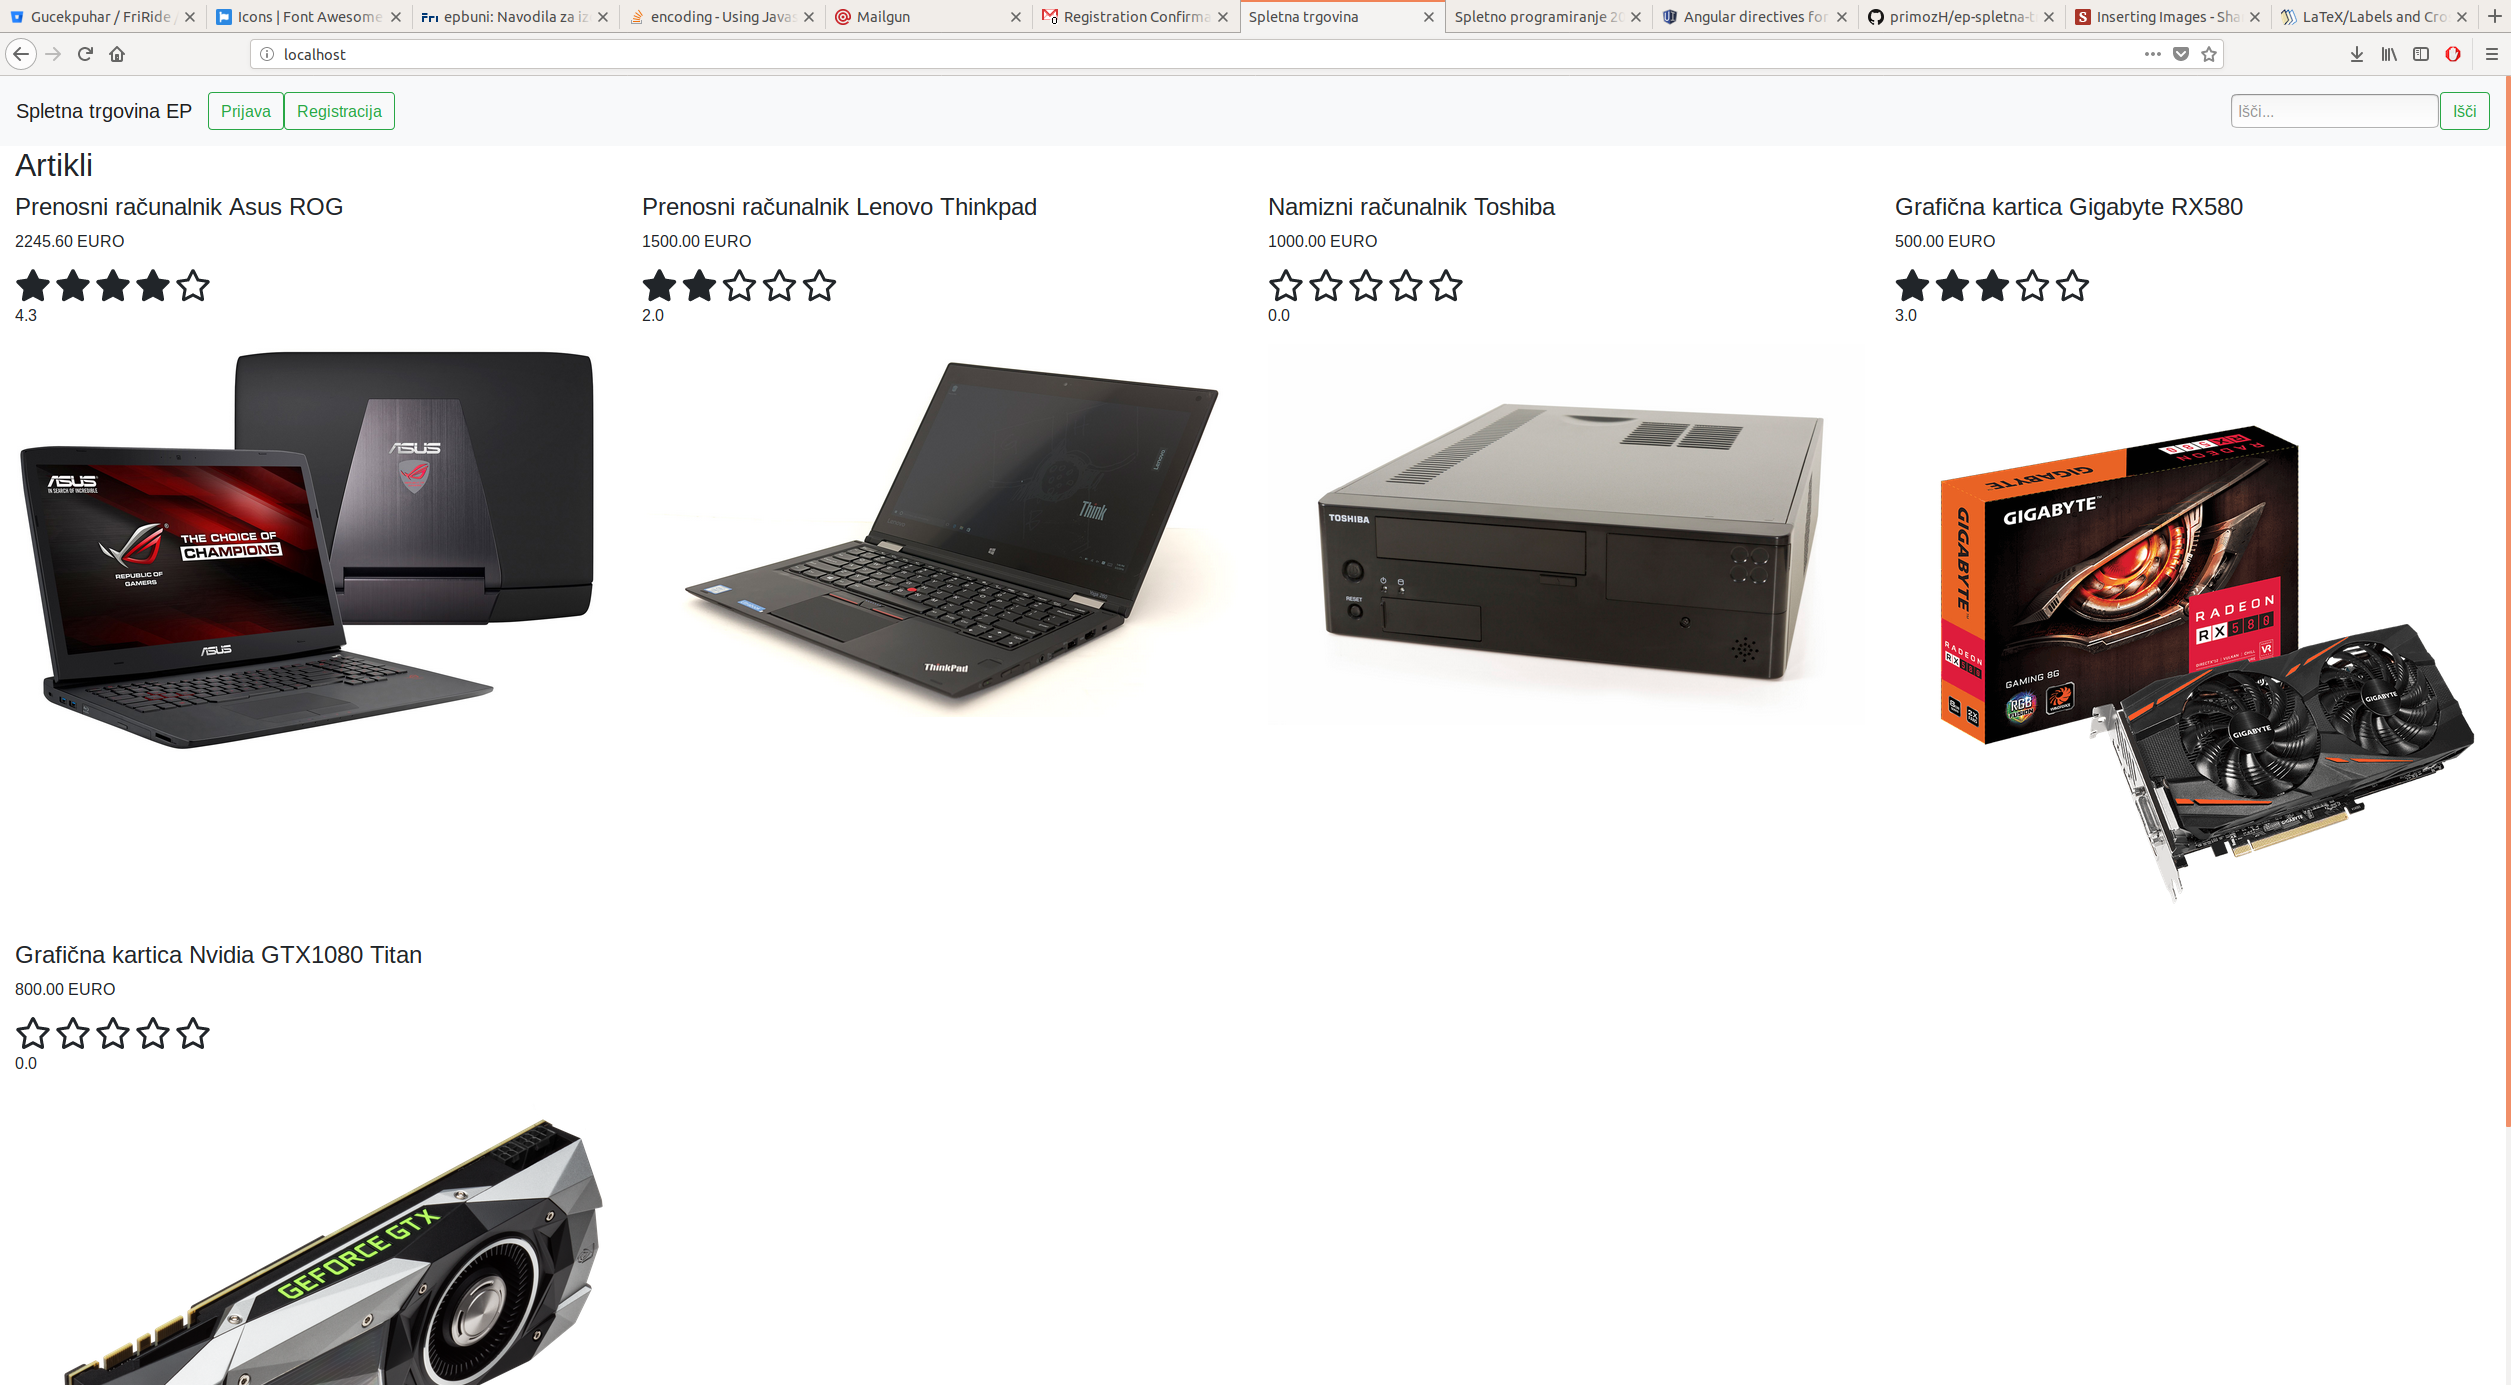
\includegraphics[width=\linewidth]{slike/splet/first_page.png}
    \caption{Začetna stran}
    \label{fig:first_page}
\end{figure}

\begin{figure}[h]
    \centering
    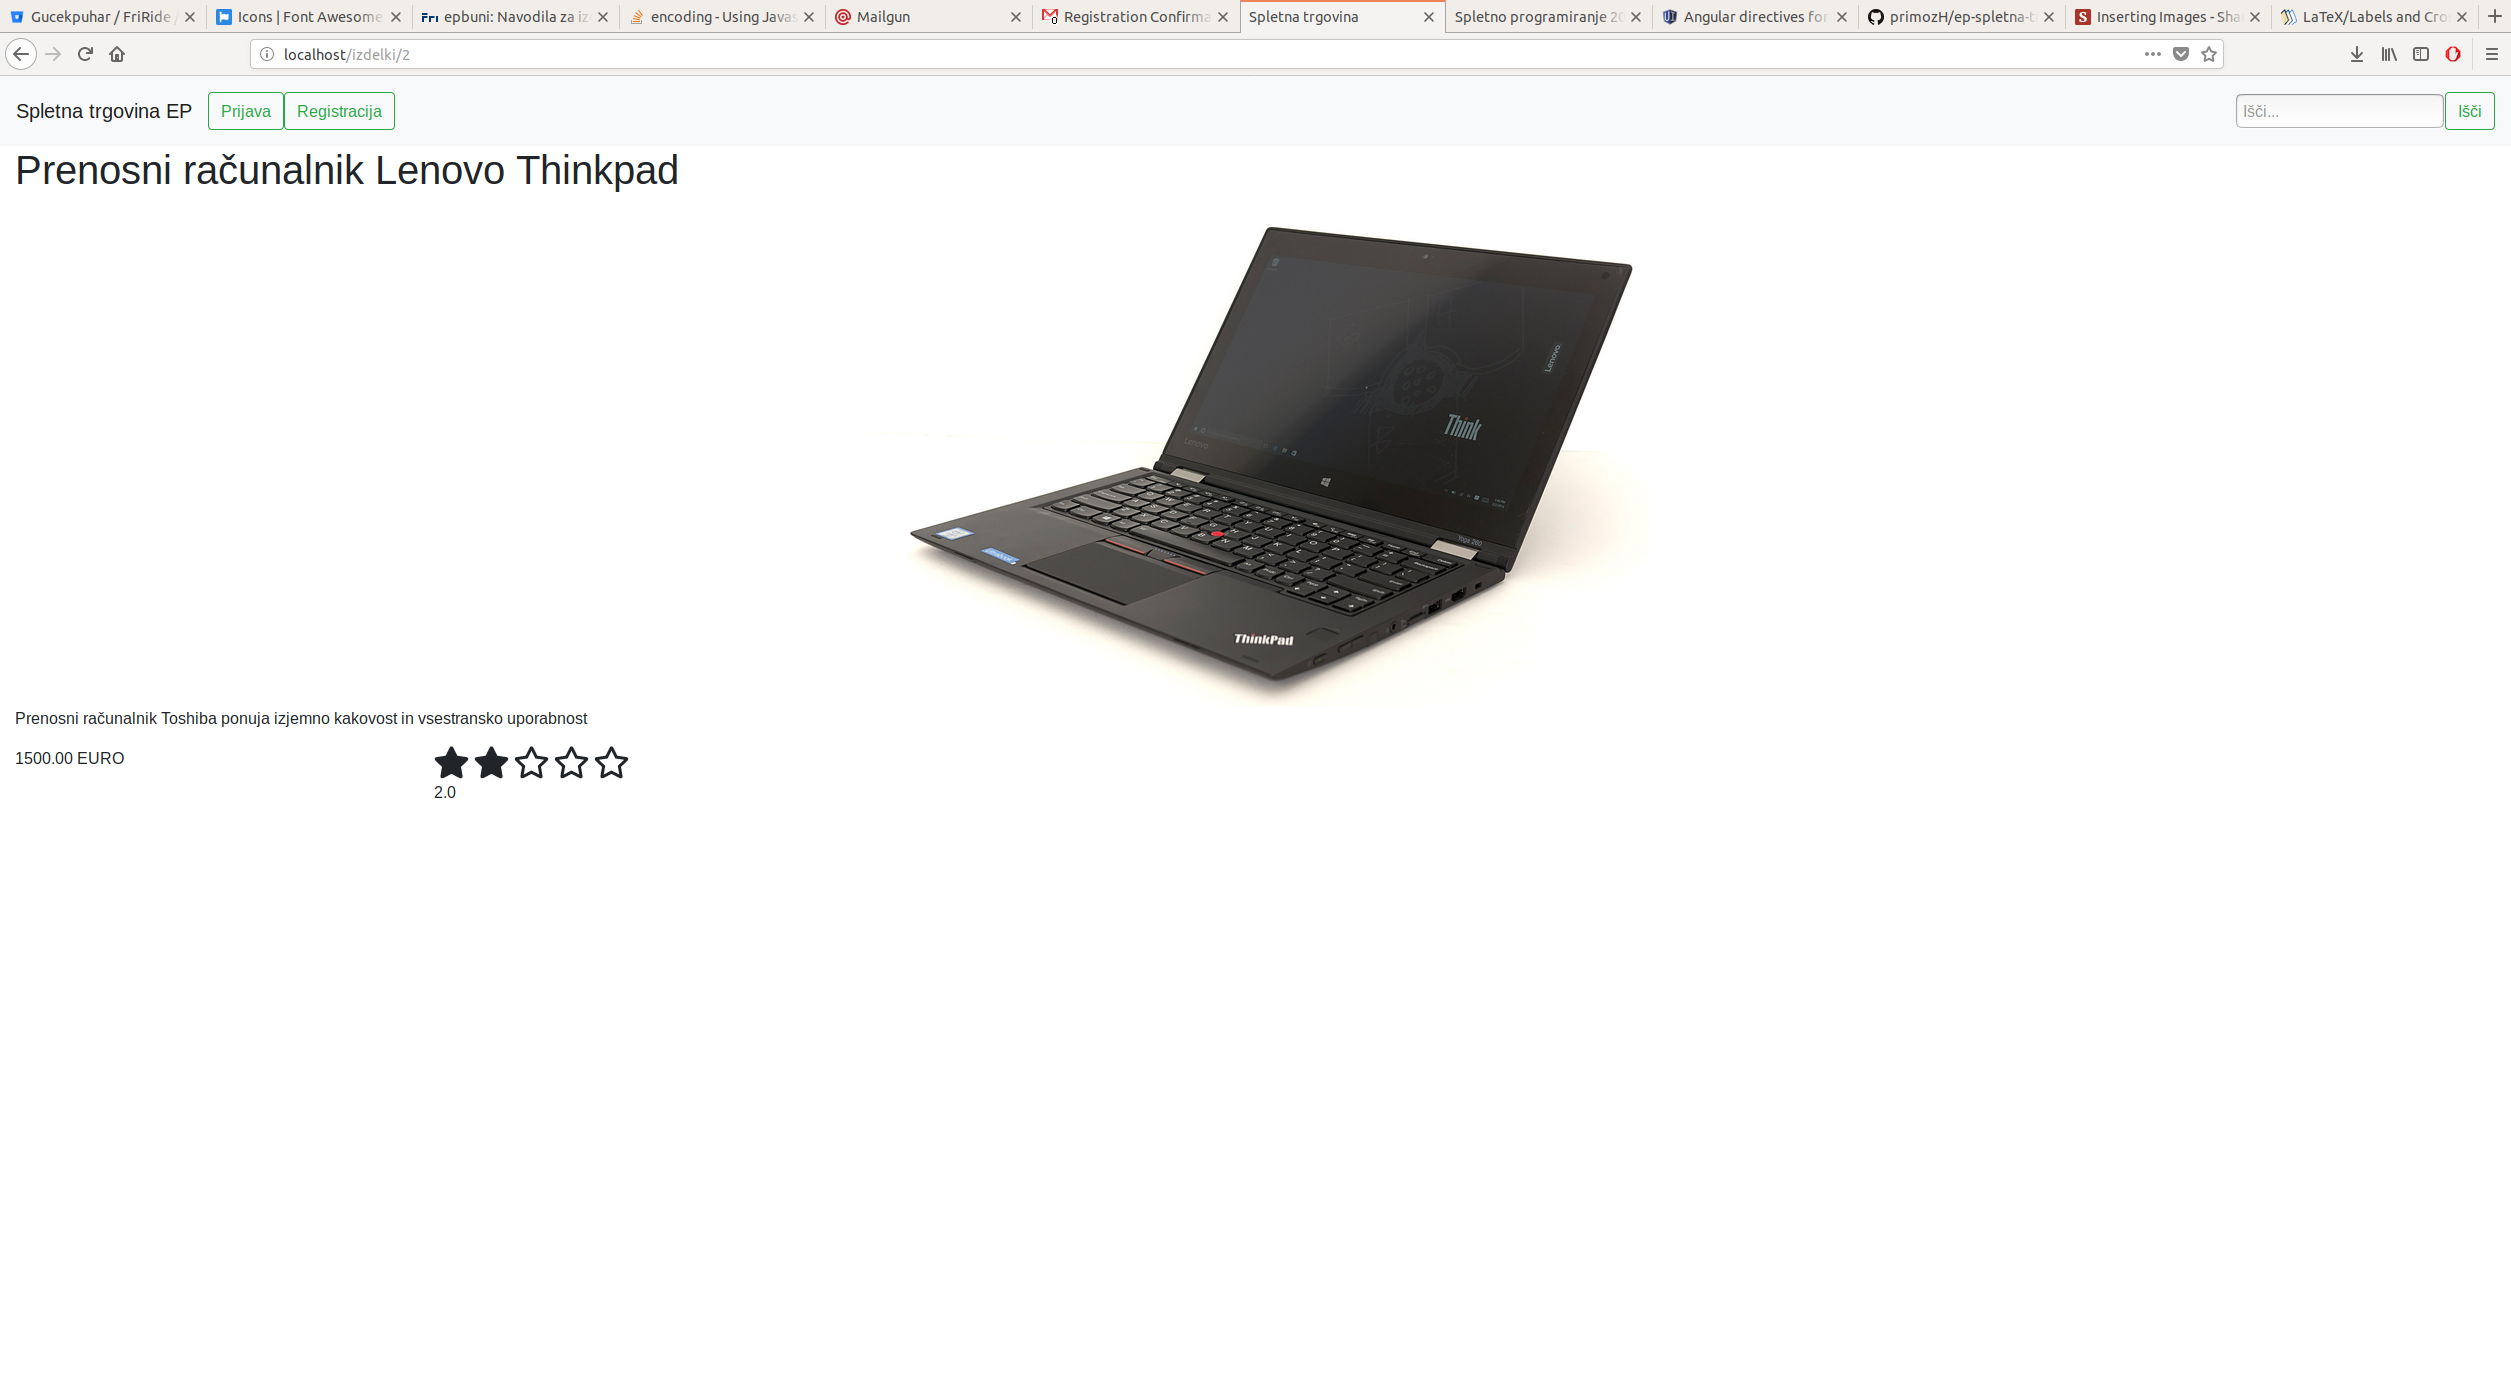
\includegraphics[width=\linewidth]{slike/splet/product_detail.png}
    \caption{Podrobnosti izdelka}
    \label{fig:product_details}
\end{figure}

\begin{figure}[h]
    \centering
    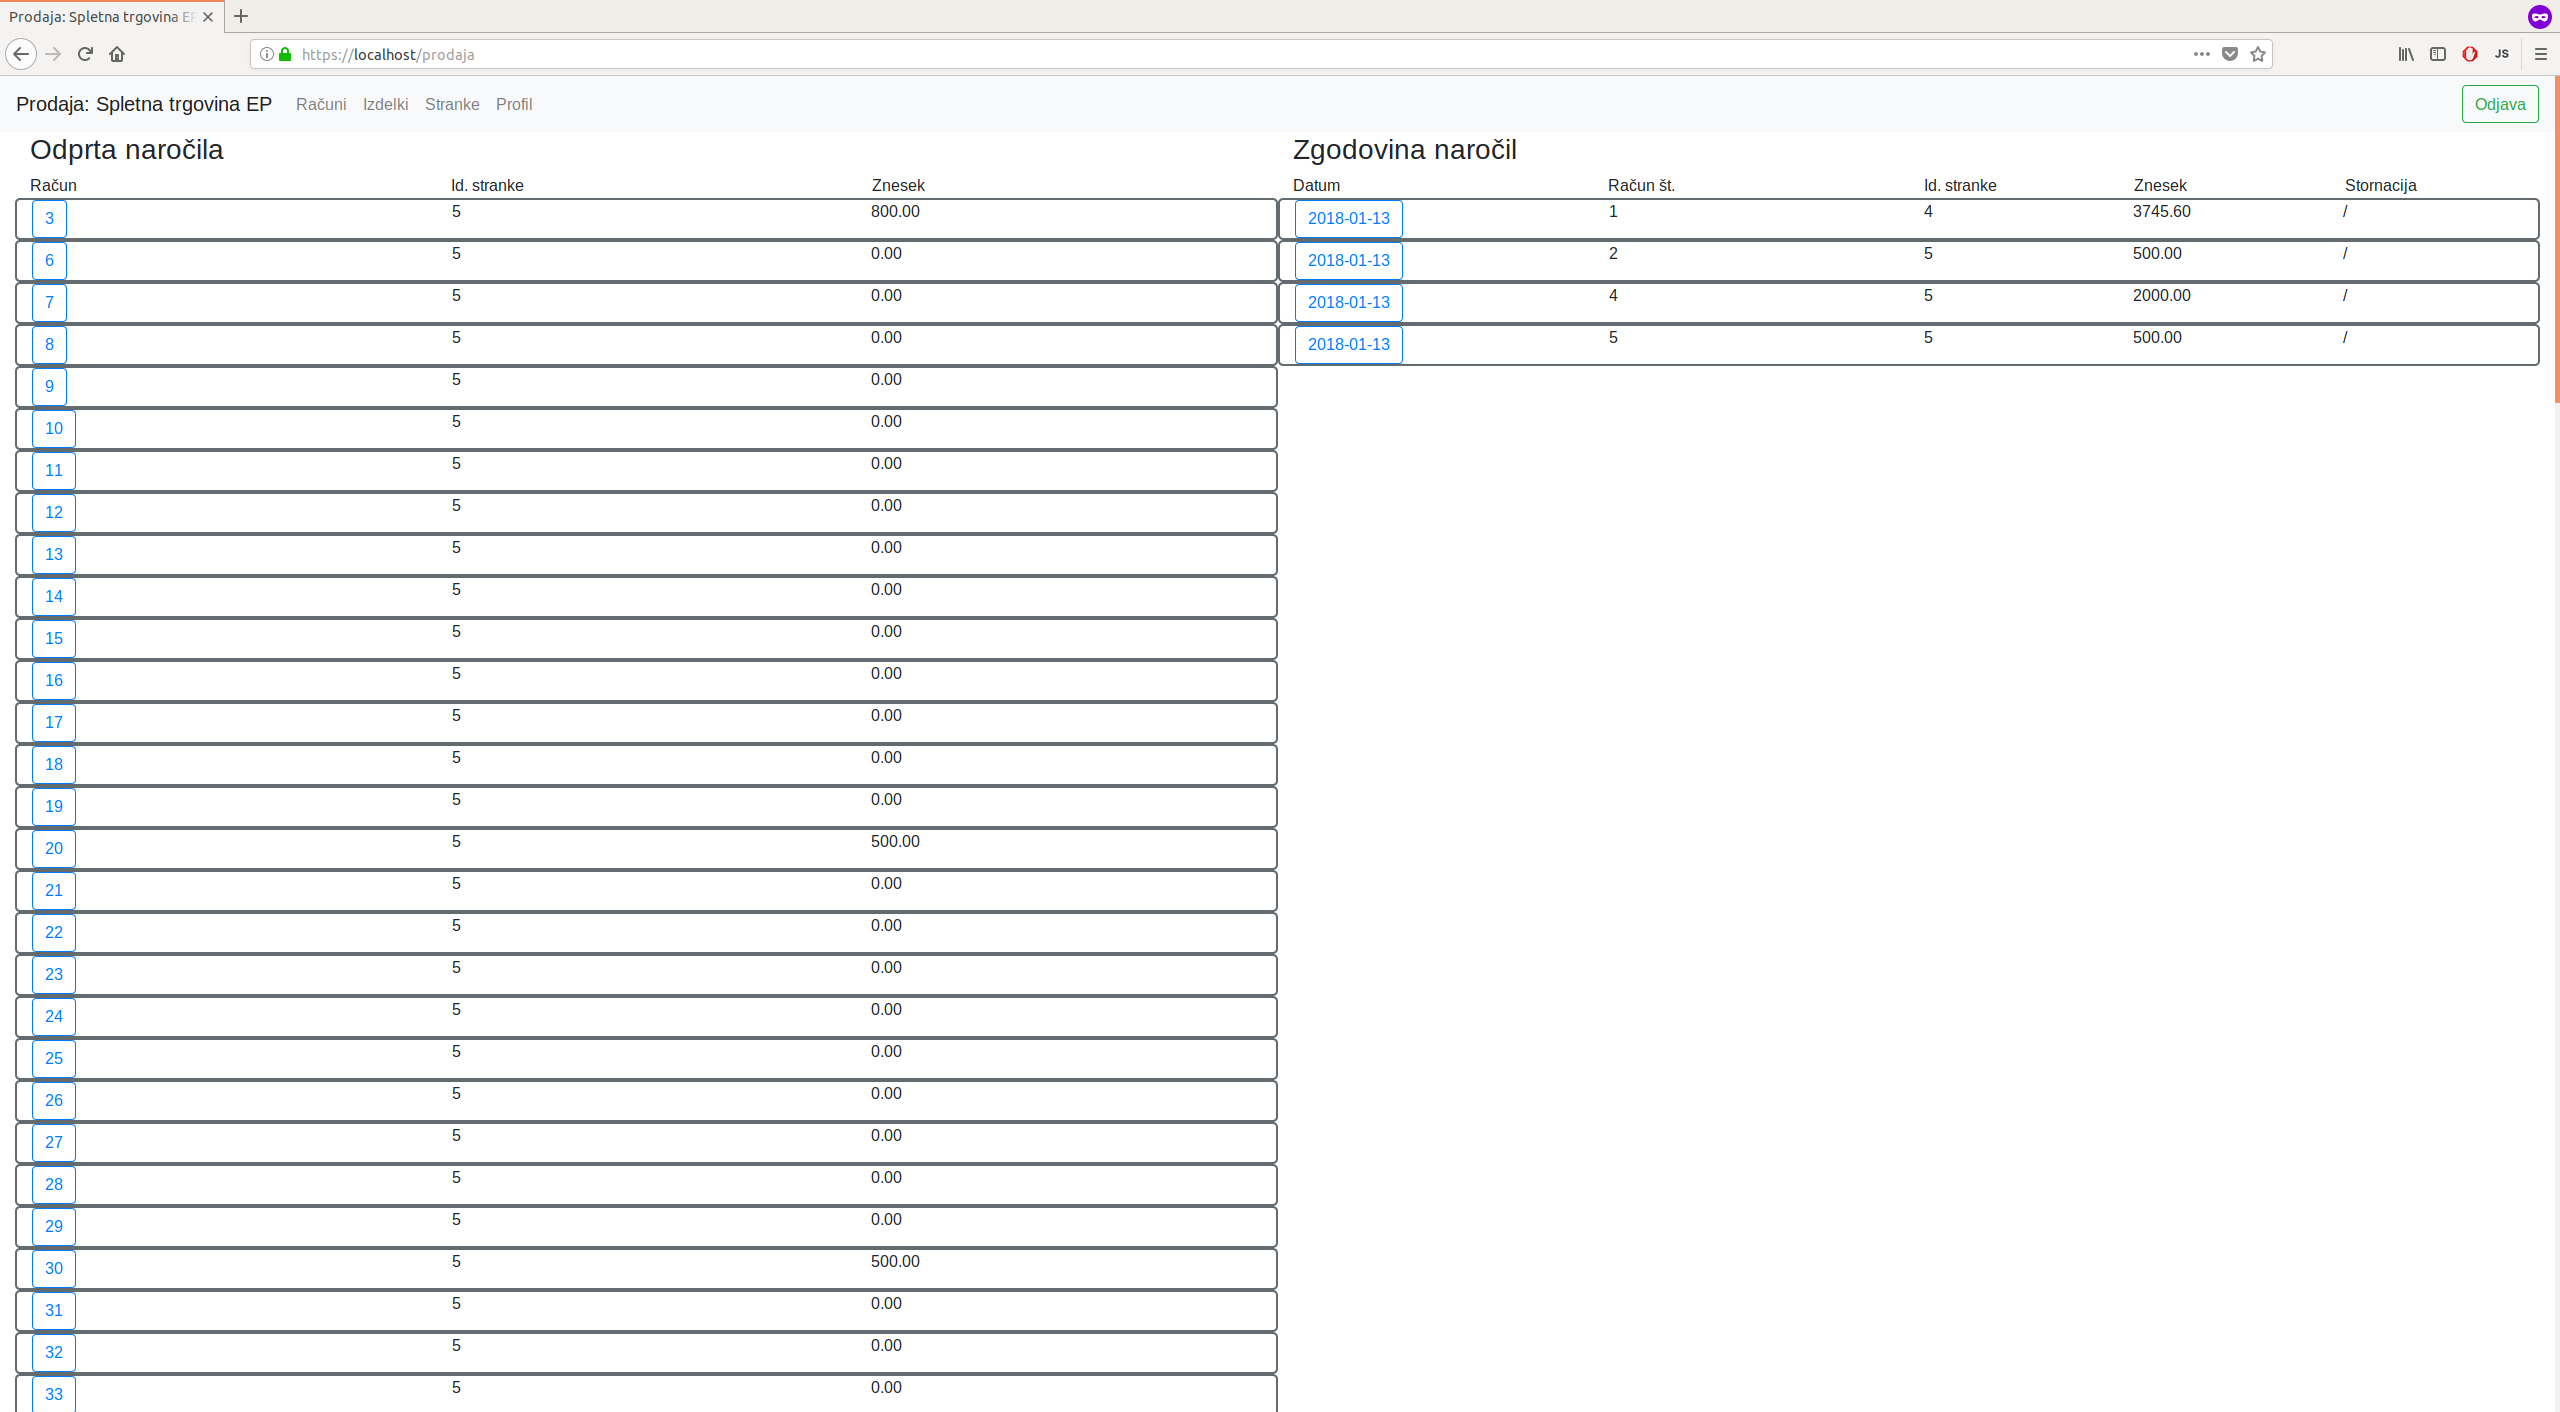
\includegraphics[width=\linewidth]{slike/splet/prodajalec_index.png}
    \caption{Začetna stran - prodaja}
    \label{fig:index_prodajalec}
\end{figure}

\begin{figure}[h]
    \centering
    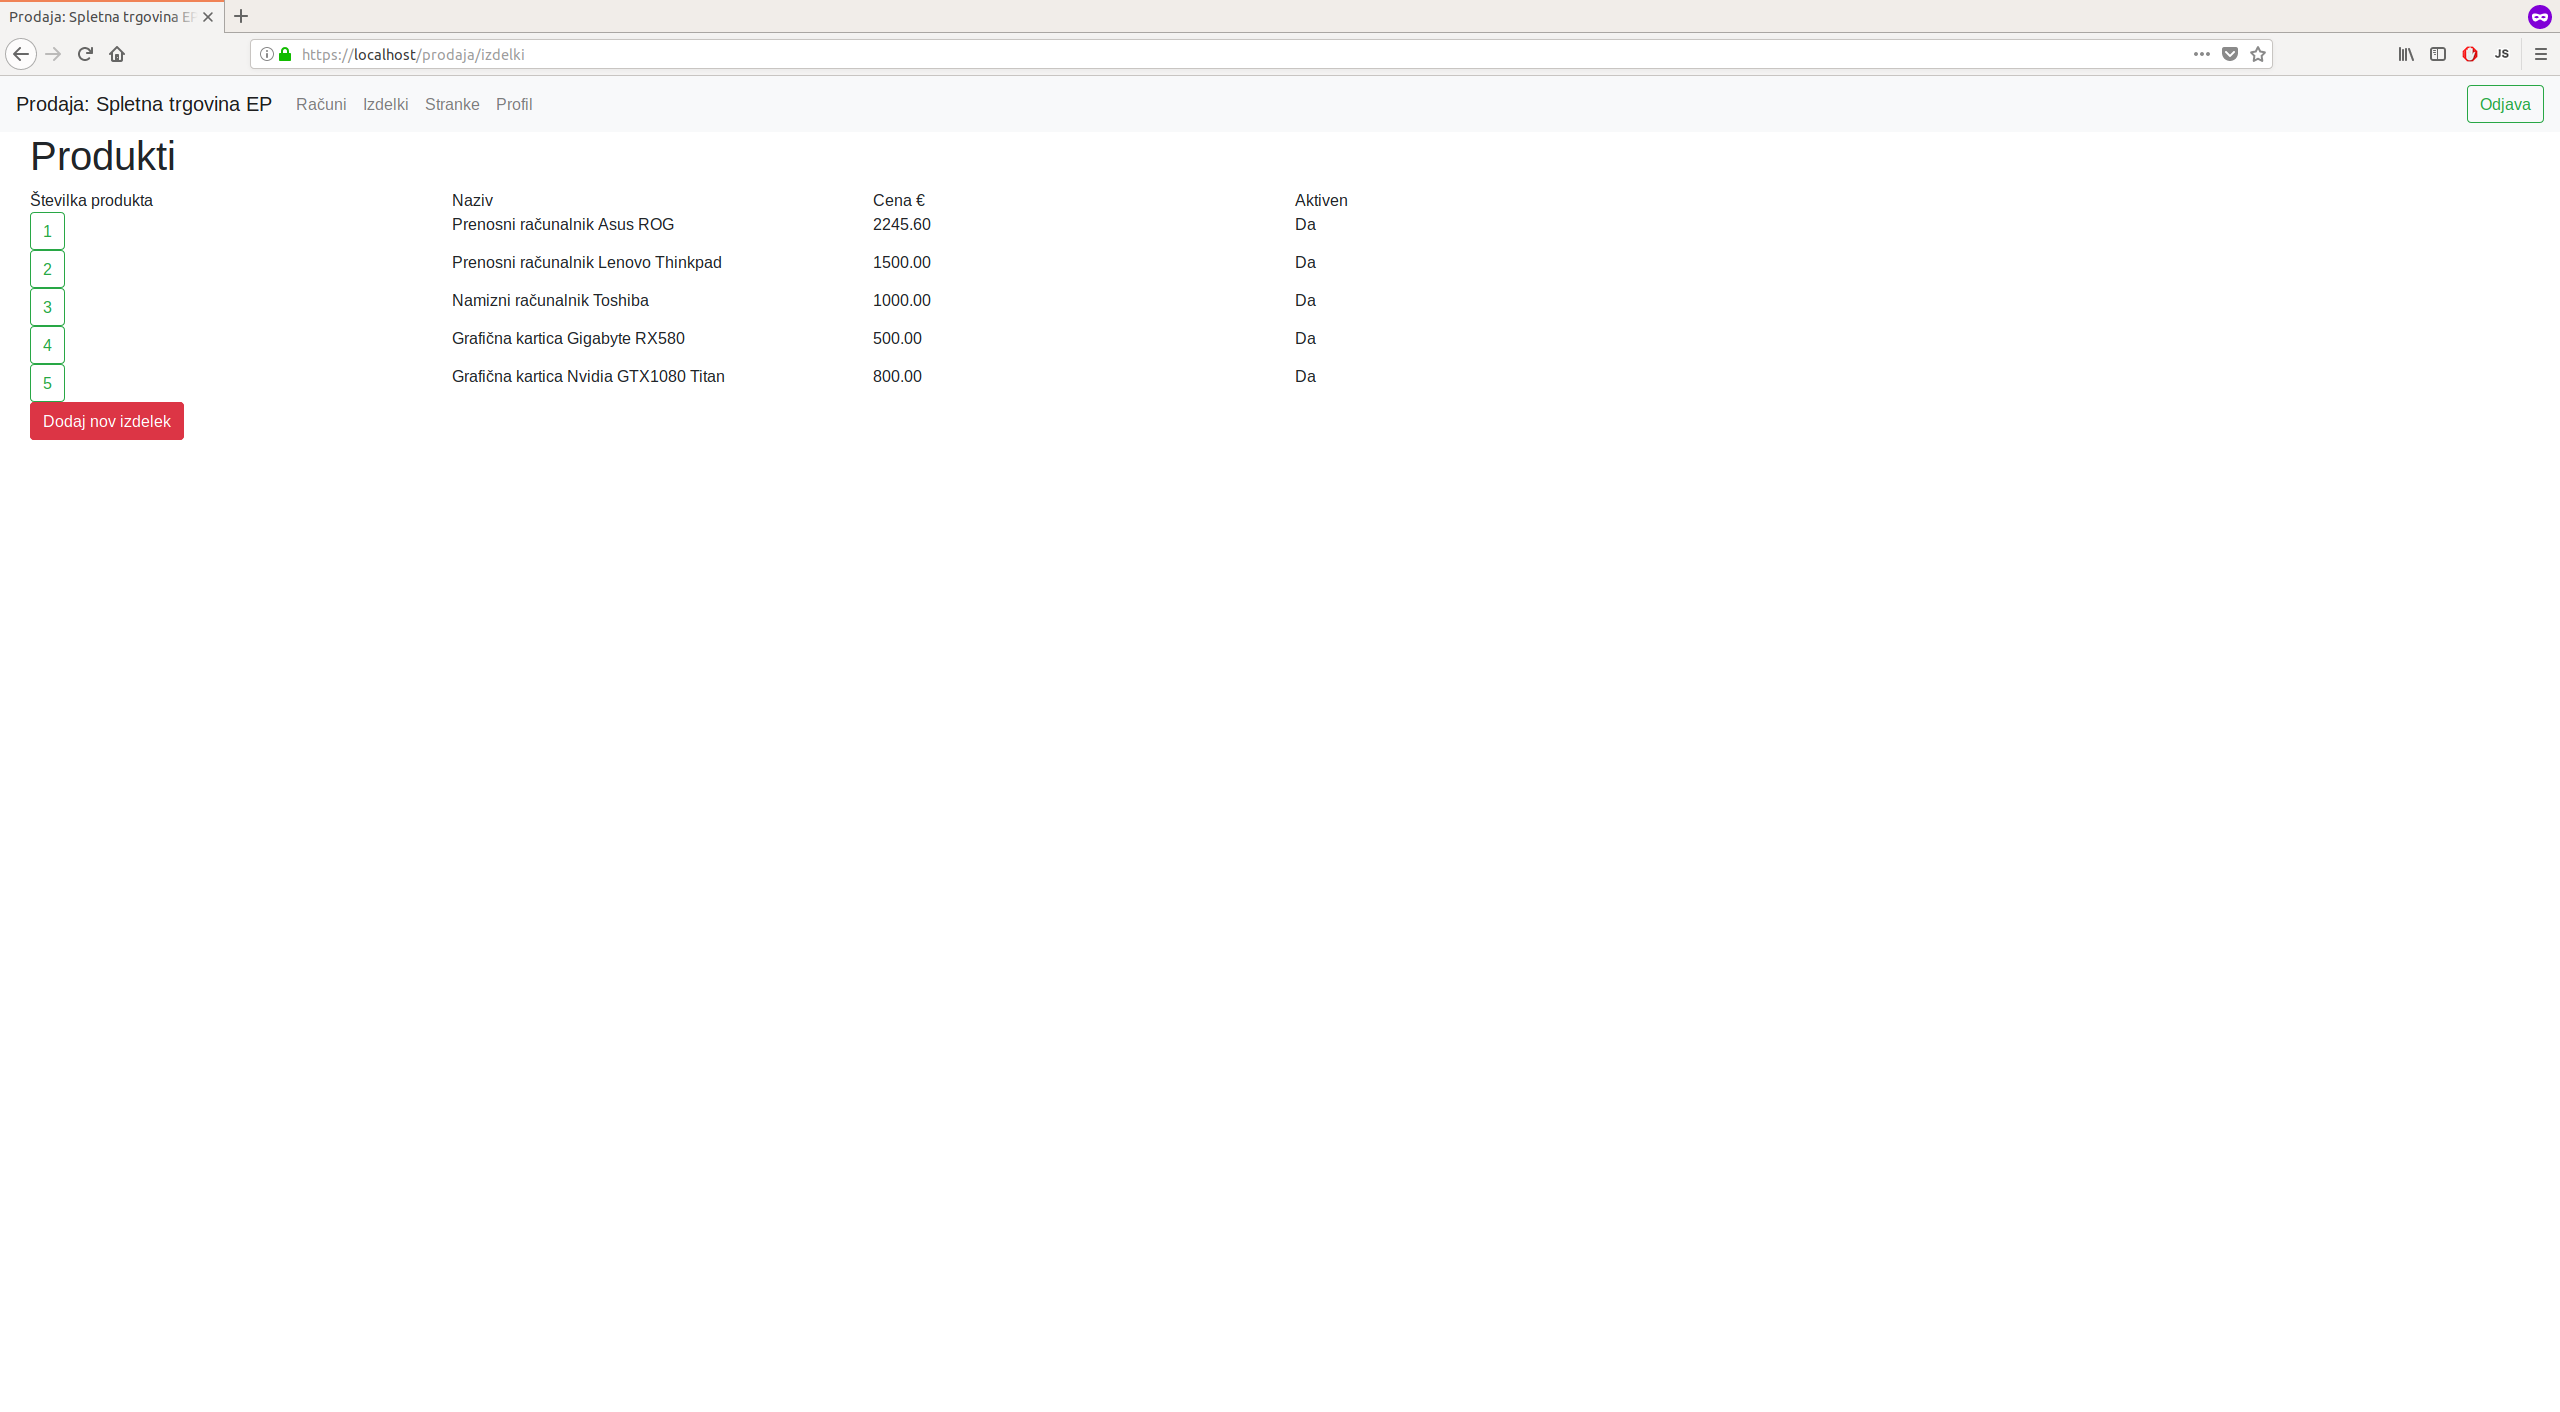
\includegraphics[width=\linewidth]{slike/splet/prodajalec_produkti.png}
    \caption{Nadzorna plošča izdelkov - prodaja}
    \label{fig:products_prodajalec}
\end{figure}
%------------------------------------------------------------------------------
\chapter{Zaslonske slike - Android aplikacija}

\begin{figure}[h]
\minipage{0.47\textwidth}
    \centering
  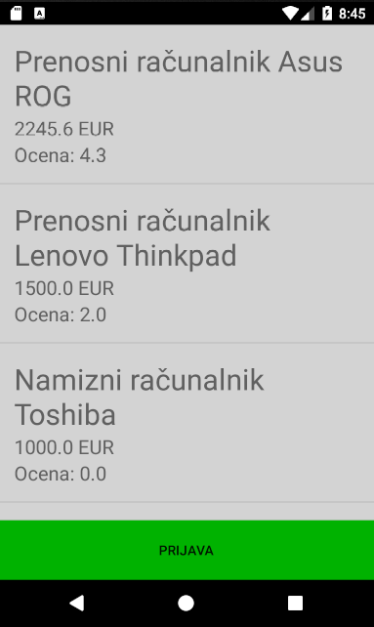
\includegraphics[scale=0.5]{slike/android/MainActivity.png}
    \caption{Pregled artiklov}
    \label{fig:main_activity}
\endminipage\hfill
\minipage{0.47\textwidth}
    \centering
  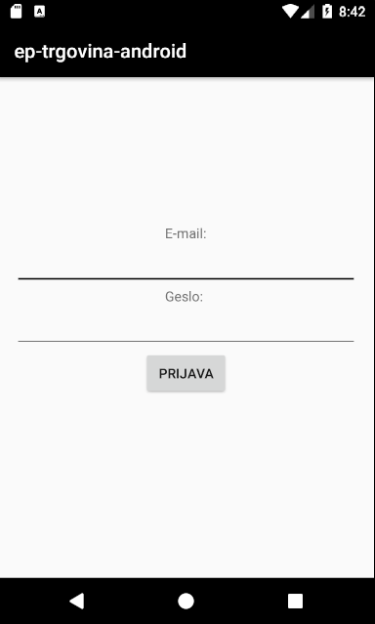
\includegraphics[scale=0.5]{slike/android/LoginActivity.png}
    \caption{Prijavno okno}
    \label{fig:login_activity}
\endminipage\hfill
\end{figure}

\begin{figure}[h]
\minipage{0.47\textwidth}
    \centering
  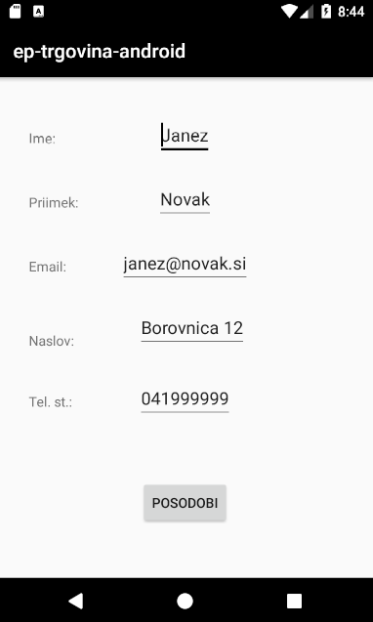
\includegraphics[scale=0.5]{slike/android/UserDataActivity.png}
    \caption{Podatki uporabnika}
    \label{fig:user_detail_activity}
\endminipage\hfill
\minipage{0.47\textwidth}
    \centering
  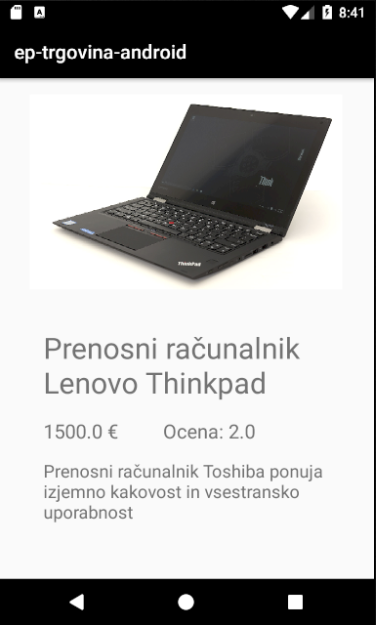
\includegraphics[scale=0.5]{slike/android/ProductDetailActivity.png}
    \caption{Podrobnosti artikla}
    \label{fig:product_detail_activity}
\endminipage\hfill
\end{figure}


% -----------------------------------------------------------------------------
% #######################
% # ZAKLJUCEK DOKUMENTA #
% #######################
\chapter{Zaključek}

Pri izdelavi seminarske naloge sva naletela na kar precej izzivov, ki sva jih bolj ali manj uspešno tudi rešila. Poseben izziv nama je predstavljalo samo učenje ogrodja Laravel in implementacija mobilnega odjemalca za Android. Laravel sam po sebi kot ogrodje omogoča ogromno nastavitev in opcij, ki se jih je potrebno zavedati in se sprva težko znajdeš že v osnovnem projektu. Pri spoznavanju okolja zelo pomaga obširna uradna dokumentacija, dostopna preko spleta \cite{bib:laravel}. Operacijski sistem Android je še toliko obsežnejši, kar predstavlja dodaten izziv, v pomoč pa je razvijalsko ogrodje Android Studio in pa uradna dokumentacija \cite{bib:android}, prav tako dostopna prek spleta.

Pri izdelavi seminarske naloge sva predvsem začutila utrip razvijalskega življenja in na lastni koži občutila, s kakšnimi problemi se srečujemo v vsakdanjiku neke razvojne ekipe. Od naloge sva odnesla veliko novega in uporabnega znanja, ki nama bo koristilo na nadaljni karierni poti.

% -----------------------------------------------------------------------------
% ##############
% # LITERATURA #
% ##############
\begin{thebibliography}{99}
\addtocounter{chapter}{1}
\addcontentsline{toc}{chapter}{\protect\numberline{\thechapter}Literatura}
\addtocontents{toc}{\protect\vspace{15pt}}

\bibitem{bib:laravel} \emph{Laravel} \url{https://laravel.com} 

\bibitem{bib:android} \emph{Android Developers} \url{https://developer.android.com/index.html}


\end{thebibliography}

% -----------------------------------------------------------------------------
% ###########
% # DODATEK #
% ###########

\end{document}
